填空:

\begin{subquestions}
    \subquestion 已知圆的半径为$r$,则其周长\key{},面积$S=$\key{}.
    \subquestion 已知甲乙两个圆的周长之比是$2:3$,那么甲乙两圆的直径之比是.
    \subquestion 如果一个扇形的圆心角是$72°$,那么它的面积相当于同半径圆面积的\key{}$\%$.
    \subquestion 如图,将一张圆形纸片剪开成甲乙两个扇形.若甲的面积是$18cm^2$,乙的面积是$12cm^2$,那么甲扇形的圆心角比乙扇形的圆心角大\key{}°.
    \subquestion 已知一个扇形的半径是$6cm$,圆心角是$120°$,则此扇形的面积是\key{}$cm$,周长是\key{}$cm^2$.
    

\end{subquestions}
\begin{center}
    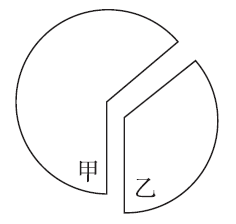
\includegraphics[height=3cm]{lib/image/MJA04000201.png}
\end{center}